\documentclass[UTF8]{ctexart}
\usepackage{amsmath}
\usepackage{diagbox}
\usepackage{textcomp}
\usepackage{graphicx}
\usepackage{float}
\usepackage{caption}
\usepackage{adjustbox}
\usepackage{subfigure}
\usepackage{geometry}
\usepackage{pifont}
\usepackage{gensymb}
\usepackage{bm}
\usepackage{tikz}
\usepackage{amstext}
\usepackage{amsfonts}

%引入代码块
\usepackage{listings}

\usepackage{xcolor}
%设置代码块格式

\definecolor{CPPGray}{RGB}{211,211,211}
\lstset{
 columns=fixed,       
 numbers=left,   % 在左侧显示行号
 numberstyle=\tiny\color{gray},% 设定行号格式
 frame=none,%none,% 不显示背景边框
 %aboveskip=1em,
 backgroundcolor=\color[RGB]{230,230,230},% 设定背景颜色
 keywordstyle=\color[RGB]{40,40,255},% 设定关键字颜色
 numberstyle=\footnotesize\color{darkgray},           
 commentstyle=\it\color[RGB]{0,96,96},% 设置代码注释的格式
 stringstyle=\rmfamily\slshape\color[RGB]{128,0,0},% 设置字符串格式
 showstringspaces=true,% 不显示字符串中的空格
 language=c++, % 设置语言
 morekeywords = {include,ull,int,double,return,static,typedef,if,else,for,long,void,class,struct,ll},                % 自加新的关键字(必须前后都是空格)
}

\begin{document}
\renewcommand{\thefootnote}{\fnsymbol{footnote}}
\newgeometry{left=2cm,bottom=3cm,right=2cm}
\linespread{1.4}
\title{\vspace{-5em}\heiti算法分析与设计基础\ \ 第八周作业\vspace{-2.5em}}
\date{}
\maketitle
\begin{center}
{\fangsong 徐浩博\quad 软件02\quad2020010108}
\end{center}


\subsection*{Problem 1}
\paragraph{a. 证明可能的接缝数是m的指数函数}\  \par
首先,我们先找到接缝数N的一个下界. 对于最上方的任意一个点,考虑到$n>2$,则它必然存在左边一列或右边一列. 我们不妨假设它存在的是左边一列,并仅考虑当前列和左列. 对于每一行,能够被选择为接缝的有两种情况,那么总共就有$2^m$种情况. 这显然是接缝数N的一个下界. \par
其次,我们考虑N的上界. 对于任何一个最上方的点,在面对下一行时最多有三种选择,即选择当前格、左下格、右下格作为接缝(由于存在边界,因此有些格子可能取不到). 考虑到每个最上方的格子走到最下部需要进行$m-1$步决策,故一个最上方格子最多对应$3^{m-1}$条可能接缝,而最上方格子有$n$个,故接缝数N的一个上界是$n3^{m-1}$.\par
结合上下界,我们可以看到,可能的接缝数是m的指数函数.
\paragraph{b. 设计动态规划算法}  \par
我们设计动态规划算法时(假设接缝从上到下进行规划),考虑每一个像素的选择:它可以从左上、上、右上三个像素获得转移(未考虑边界的情况下),转移的损失记为d,那么第i行j列的像素动态规划方程可以写作:
\[A[i][j] = min(A[i - 1][j - 1], A[i - 1][j], A[i - 1][j + 1]) + d[i][j];\]
其中A[i][j]表示终点为第i行j列的像素其上方的累计最小损失. 初始条件为A[1][i] = 0.\par
我们将之写成伪代码:
\begin{lstlisting}
    let all the elements of A = 0
    let all the elements of pre = 0 
	for(int i = 1; i < h - 1; i++) //height
		for(int j = 1; j < w - 1; j++) //weight
	{
		
		A[i][j] = A[i - 1][j] + d[i][j]
		pre[i][j] = (i, j)
		if (j < w - 2 and A[i - 1][j + 1] + d[i][j] < A[i][j]) 
		{
			A[i][j] = A[i - 1][j + 1] + d[i][j] 
			pre[i][j] = (i - 1, j + 1)
		}
		if (j > 1 and dp[i - 1][j - 1] + d[i][j] < A[t]) 
		{
			dp[t] = dp[i - 1][j - 1] + d[i][j] 
			pre[i][j] = (i - 1, j - 1)
		}
	}
    minimum_loss = min{A[h - 1][1] ... A[h - 1][w - 2]}
\end{lstlisting}
我们看到计算的复杂度瓶颈在于内外嵌套的两层循环,因此对于一次seam-carving来说,复杂度是$\Theta(mn)$.
\paragraph{c. 实验报告}\  \par
\subsubsection*{摘要}
{\kaishu\normalsize  seam-carving算法是一种基于动态规划的图像压缩算法. 本实验意图对真实的RGB图片,结合sobel算子识别边界并进行seam-carving压缩. 具体来说,我们会将读入一张24位BMP图片,并利用算法将它的长宽压缩到原来的1/2,并且将图片输出,这样可以直观检验我们的seam-carving压缩成果.}
\subsubsection*{关键词:seam-carving\ \ 动态规划\ \ sobel算子\ \  BMP格式\vspace{1.5em}}

\section*{1\ \ \ 实验环境}
操作系统:Windows 10\par
编译器:g++ (gcc 6.3.0)\par
处理器:Intel Core i7-10750H 六核CPU @ 2.60GHz\par
编程语言:C++
\section*{2\ \ \ 算法分析}
具体的动态规划方法已经在前面叙述过,这里不再赘述. 我们要将长宽均压缩到原来的一半,可以先对宽进行seam-carving压缩n/2次,然后将图片翻转90度再对长(翻转后是宽)压缩m/2次,再翻转回来即可.\par
计算实际复杂度时,先看翻转前,计算复杂度为$\Theta(mn)+\Theta(m(n-1))+\cdots + \Theta(m(n/2 + 1)) = \Theta(mn^2)$;翻转后为$\Theta(mn/2)+\Theta((m-1)n/2)+\cdots + \Theta((m/2 + 1)n/2) = \Theta(m^2n)$. 因此总复杂度为$\Theta(mn(m+n))$.
\section*{3\ \ \ 实验设计思路}
程序分为读入、动态规划、输出三个部分. 由于我们只考虑24位BMP图,因此读入时先读入文件头,然后分像素保存每个像素的RGB对应值. 动态规划阶段,先正着进行n/2次seam-carving;然后翻转90度,进行m/2次;最后翻转回来,得到的就是长宽均压缩一半的图片. 输出阶段,我们将输入的文件头中长宽进行更改并输出,然后分像素输出压缩后的图片每个像素对应的RGB值即可.\par
值得注意的是,动态规划阶段,我们采用的损失权重是sobel算子计算出来的,算子的值越大,说明该像素越可能是边界,因此越不应该被裁剪;由此可以将每个像素先转化为灰度像素,然后进行sobel算子运算.
\section*{4\ \ \ 结果展示}
压缩前的图片如图(1200$\times$800):
\begin{figure}[H]\begin{center}
	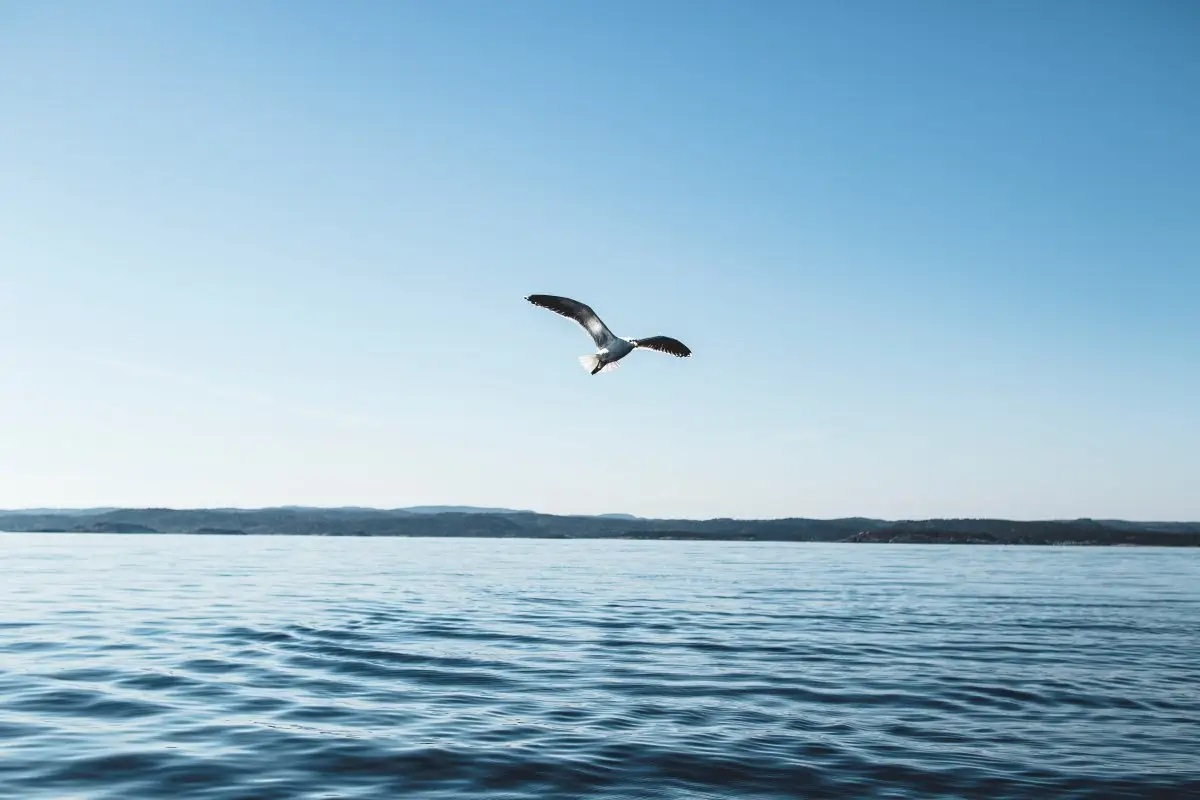
\includegraphics[scale = 0.5]{1.jpg}\end{center}
\end{figure}
压缩后的图片如图(600$\times$400):
\begin{figure}[H]\begin{center}
	
\includegraphics[scale = 0.5]{2.jpg}\end{center}
\end{figure}
\section*{5\ \ \ 总结}
在实验中,我们利用seam-carving算法对RGB图像的长宽进行了压缩,可以看到,压缩后的图片基本保留了原有图片的重要信息,但长宽分别压缩为了原来的一半. 但我们也需要看到,压缩比较大时,该算法的复杂度是很高的,而且压缩的图像还是存在畸变、失真等问题,这些都有待更有效更快捷的其他算法进行改进.

\subsection*{Problem 2}
本题中,我们采用的贪心策略是,首先对所有活动按照开始时间从小到大进行排序. 理想的排序时间开销为O(nlogn). 下面我们再开辟一个H数组记录新开辟的教室,H初始为空. 对于排序好的活动从小到大依次进行如下贪心操作:对于第i项活动,检查现有开辟的教室H中是否存在结束时间早于活动i开始时间的活动,如果存在教室j满足,则在教室j进行活动i,并将H[j]置为i的结束时间;否则H中加入一个教室,让它的值为i的结束时间. 考虑到H可以用小顶堆维护,因此我们将H设为小顶堆,这样对n个教室遍历,每次访问堆顶/插入一个元素,总复杂度为O(nlogn). 综合以上两点,总复杂度为O(nlogn).\par
下面我们采用数学归纳法证明这种贪心算法能够得到正确答案. 我们假设这种算法在做第i个活动的决策后,总能使编号1-i的活动利用最少的教室. i=1时,显然必须开辟一个新教室,最少的教室为1,算法正确. 假设i=k时也成立. 则i=k+1时,活动i有两种决策可能. i)可以不开辟新教室,则与i=k相比,总教室数不变,由归纳假设,1-k采用了最少的教室num,1-k+1需要的教室数显然不小于num,我们的贪心决策没有增加新教室,则num也是1-k+1需要的最少教室数. ii)必须要开辟一个新教室,在这种情况下,所有已开辟的num个教室最后一个活动(记为$a_1 ... a_{num}$)结束时间必然都大于第i个活动的开始时间. 我们采用反证法证明num+1是1-k+1个活动所需要的最小教室数. 假设num个教室足够这k+1个活动开展,考虑到i与$a_1 ... a_{num}$均不兼容,那么$a_1 ... a_{num}$中必然有两个活动$a_k, a_l$兼容,这样才能腾出教室给i活动,而$a_k, a_l$兼容则说明其中一个活动开始时间大于等于另一个结束时间(不妨设$a_k.finish\_time\leq a_l.start\_time$),而由i序号小于$a_l$有$i.start\_time \geq a_l.start\_time$,因此有$a_k.finish\_time \leq i.start\_time$
. 但是由i与$a_k$不兼容得$a_k.finish\_time > i.start\_time$,推出矛盾,因此num+1是活动1-k+1需要的最小教室数. 结合数学归纳法,我们证明了该算法的正确性.\par

该算法的伪代码为:
\begin{lstlisting}
GREEDY_ALGORITHM:
	let A[1 ... n] be an array of tuples (start_time, finish_time)
	sort A[1 ... n] from the smallest to the largest by start_time 
	let H be a minHeap which is empty at first
	for i from 1 to n:
		if H is empty or H.top > A[n].start_time:
			H.insert(A[n].finish_time)
		else:
			H.extract_min
			H.insert(A[n].finish_time)
	return H.size
\end{lstlisting}
\end{document}
